\section{Miscellaneous topics}

\begin{frame}{Adversarial attacks}
\begin{columns}
	\begin{column}{.5\textwidth}
		\begin{figure}
			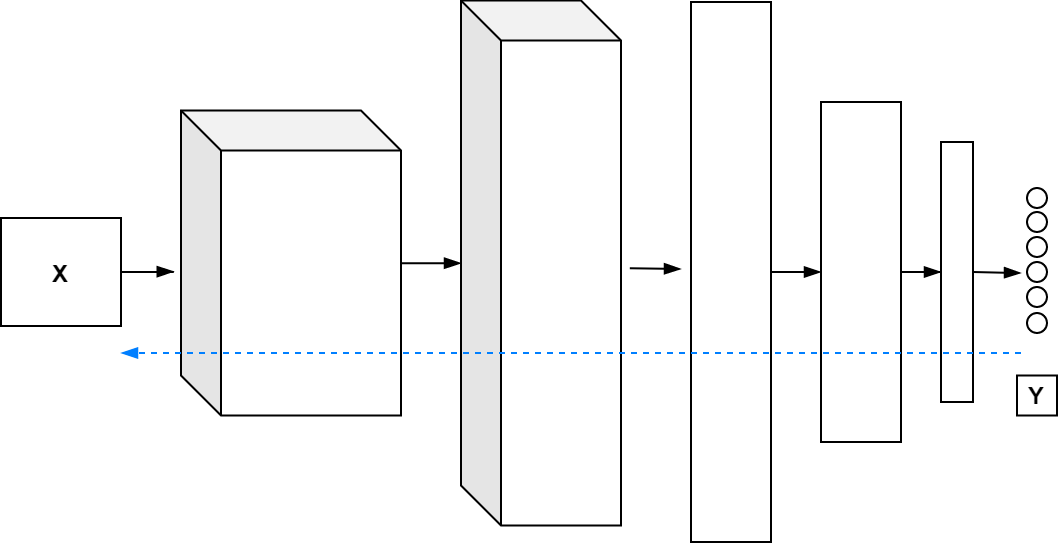
\includegraphics[width=.8\textwidth]{figures/adverserial-net}
			\caption*{Classification network}
		\end{figure}
	\end{column}
	\begin{column}{.5\textwidth}
		Let $\hat{y}$ be the desired label,  $y$ be the predicted label.
		\begin{itemize}
			\item  Consider  the loss function $L=D_1(\hat{y},y)$ 
			\item  If $\hat{x}$ is the desired image, consider another loss function 
				$L=D_1(\hat{y},y) + \lambda D_2(\hat{x},x) $
		\end{itemize}
	\end{column}
\end{columns}
\end{frame}
\begin{frame}{Adversarial examples}
\begin{columns}
\begin{column}{.5\textwidth}
	\begin{figure}
		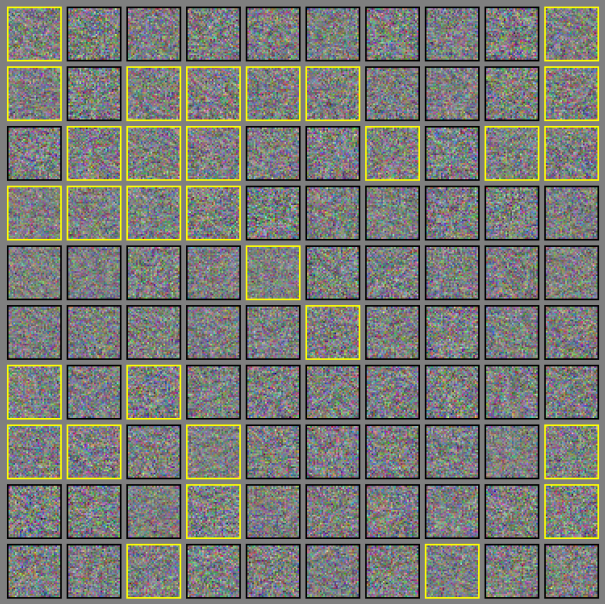
\includegraphics[width=.8\textwidth]{figures/adverserial-example-1}
		\caption*{\tiny{I. Goodfellow, J. Shlens, and C. Szegedy, Explaining and
				harnessing adversarial examples," in International Conference on Learning Representations, 2015.}}
	\end{figure}
\end{column}
\begin{column}{.5\textwidth}
	\begin{figure}
		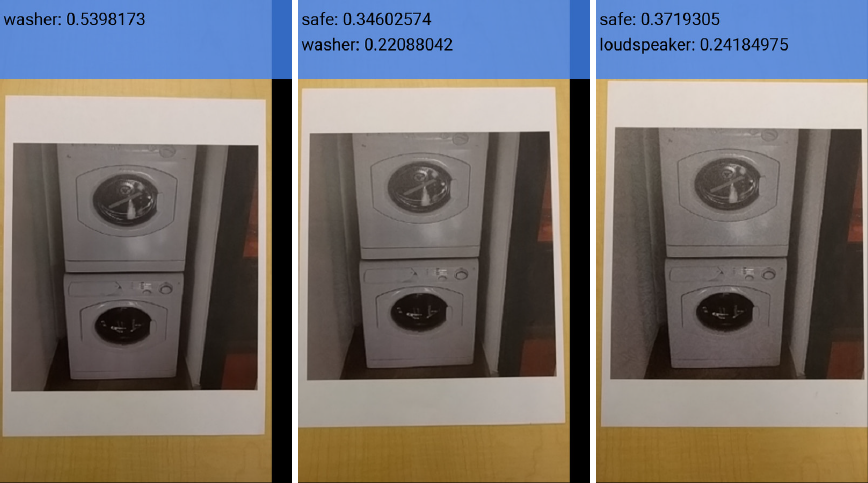
\includegraphics[width=1\textwidth]{figures/adverserial-example-2}
		\caption*{\tiny{A. Kurakin, I. Goodfellow, and S. Bengio, Adversarial
				examples in the physical world," ICLR Workshop, 2017.}}
	\end{figure}
	What kinds of attacks can you think of?
\end{column}
\end{columns}
\end{frame}

\begin{frame}{Generative adversarial networks - intuition}
\begin{center}
	\begin{figure}
		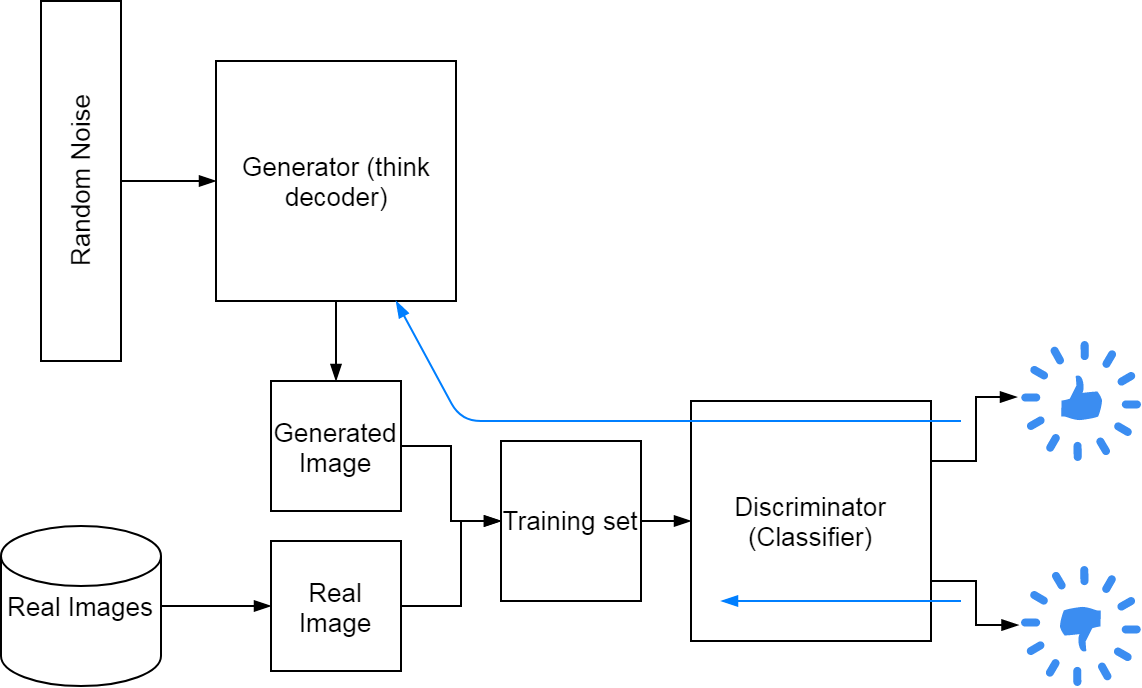
\includegraphics[width=.8\textwidth]{figures/gan-simple}
		\caption*{Learning data distribution}
	\end{figure}
\end{center}
\end{frame}

\begin{frame}{Attention - intuition} 
\begin{center}
	\begin{figure}
		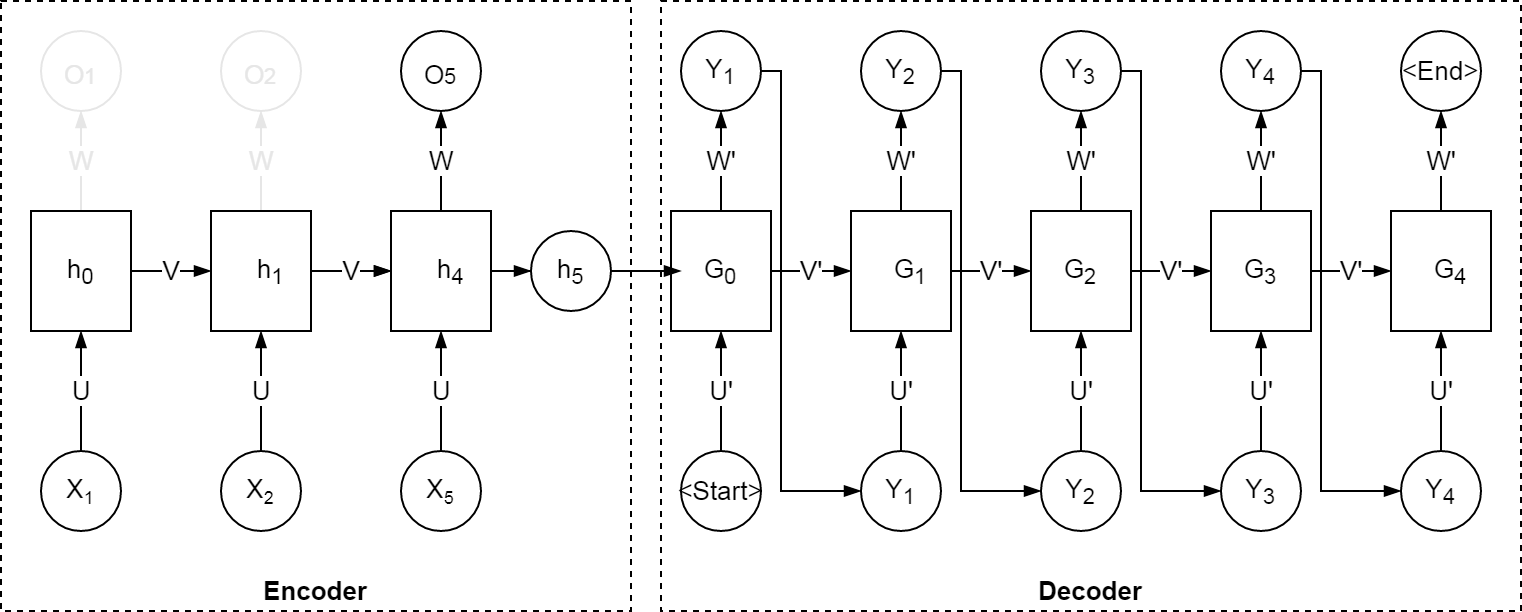
\includegraphics[width=1\textwidth]{figures/rnn_seq_2_seq_encoder_decoder}
		\caption*{{Sequence to sequence encoder-decoder network}}
	\end{figure}
\end{center}
\end{frame}